\chapter{Biogeochemische kringlopen}\label{ch:b2:biogeochemical-cycles}

In maart 1958 zette een jonge chemicus, Charles Keeling, een infrarood
gasanalysetoestel aan op de noordflank van de Mauna Loa, op Hawaï, drie en een
halve kilometer boven de Stille Oceaan, waar de lucht zo goed gemengd is als
lucht maar kan zijn. Hij had verwacht een constante te meten; binnen een jaar
had hij een zaagtand --- koolstofdioxide dat elke winter steeg en elke zomer
daalde terwijl de bossen van het noordelijk halfrond uit- en inademden --- en
binnen enkele jaren een helling onder de zaagtand die sindsdien niet is
gestopt. De keelingcurve is de ademhaling van de biosfeer, van buitenaf
gezien, met een koortscurve eroverheen getekend. Dit hoofdstuk gaat over de
kringlopen die de curve vastlegt: waar de koolstof, stikstof, fosfor en
zwavel van levende wezens zijn opgeslagen, hoe snel ze tussen \omterm{def:b2:biogeochemical-cycles:reservoir}{reservoirs}
bewegen, wat die snelheden bepaalt --- meestal de stofwisselingen van
\cref{ch:b2:microbial-metabolism} --- en wat één soort in tweehonderd jaar met
elke kringloop heeft gedaan.

\section{Reservoirs, fluxen en verblijftijden}

\begin{definition}[Reservoir, flux, verblijftijd]\label{def:b2:biogeochemical-cycles:reservoir}
\index{reservoir}\index{flux}\index{verblijftijd}\index{stationaire toestand}\index{biogeochemische kringloop}
Een \emph{biogeochemische kringloop} is de beweging van een element tussen
\emph{reservoirs} (de atmosfeer, de oceaan, bodems, levende biomassa,
gesteenten) door \emph{fluxen}, gemeten in massa per jaar. Een reservoir met
massa $M$ en totale uitstroom $F$ heeft een \emph{verblijftijd}
$\tau = M/F$, de gemiddelde tijd die een atoom erin doorbrengt; in
\emph{stationaire toestand} is de instroom gelijk aan de uitstroom en is $M$
constant. De kringlopen zijn gekoppeld via de stoichiometrie van het leven ---
de \emph{redfieldverhouding} van marien plankton, $\mathrm{C:N:P} =
106:16:1$ in atomen --- zodat de aanvoer van het schaarste element
bepaalt in welk tempo alle andere worden opgenomen.
\end{definition}

\begin{theorem}[Het model met één box]\label{thm:b2:biogeochemical-cycles:box}
\index{boxmodel}\index{relaxatietijd}
Als een \omterm{def:b2:biogeochemical-cycles:reservoir}{reservoir} zijn inhoud verliest met een snelheid evenredig met wat het
bevat, $F_{\text{uit}} = M/\tau$, en een constante instroom
$F_{\text{in}}$ ontvangt, dan geldt
\[
\frac{\mathrm{d}M}{\mathrm{d}t} = F_{\text{in}} - \frac{M}{\tau},
\qquad
M(t) = M^{*} + (M_0 - M^{*})\,e^{-t/\tau}, \qquad M^{*} = F_{\text{in}}\tau :
\]
en het \omterm{def:b2:biogeochemical-cycles:reservoir}{reservoir} relaxeert naar een \omterm{def:b2:biogeochemical-cycles:reservoir}{stationaire toestand} evenredig met zijn
aanvoer, met de \omterm{def:b2:biogeochemical-cycles:reservoir}{verblijftijd} als tijdconstante. Een stapsgewijze toename van de
aanvoer verhoogt de \omterm{def:b2:biogeochemical-cycles:reservoir}{stationaire toestand} evenredig, en het \omterm{def:b2:biogeochemical-cycles:reservoir}{reservoir} volgt
binnen enkele $\tau$: een voorraad met een \omterm{def:b2:biogeochemical-cycles:reservoir}{verblijftijd} van dagen
(atmosferisch ammoniak, het nitraat van een meer in de lente) volgt zijn
bronnen; een voorraad met een \omterm{def:b2:biogeochemical-cycles:reservoir}{verblijftijd} van eeuwen (koolstof in de diepzee,
organisch materiaal in de bodem) integreert ze, en de verstoring van een
trage voorraad duurt langer dan de verstoring die haar veroorzaakte.
\end{theorem}
\begin{proof}
De vergelijking is lineair met constante coëfficiënten: de \omterm{def:b2:biogeochemical-cycles:reservoir}{stationaire toestand}
$M^{*}$ maakt het rechterlid nul, en de afwijking $m = M - M^{*}$
voldoet aan $\dot m = -m/\tau$, dus $m = m_0 e^{-t/\tau}$. Als een \omterm{def:b2:biogeochemical-cycles:reservoir}{reservoir}
meerdere uitstromen heeft, wordt $\tau$ door hun som bepaald, $1/\tau = \sum_i
1/\tau_i$: de snelste afvoer overheerst.
\end{proof}

\section{De koolstofkringloop}

\begin{proposition}[Het koolstofbudget]\label{prop:b2:biogeochemical-cycles:carbon}
\index{koolstofkringloop}\index{atmosferische fractie}\index{koolstofput}\index{keelingcurve}
In gigatonnen koolstof (\unit{GtC}, $10^{12}$~kg) zijn de
belangrijkste \omterm{def:b2:biogeochemical-cycles:reservoir}{reservoirs} de atmosfeer (ongeveer 880 in de jaren 2020, 590
vóór de industrie), landplanten (450), bodems (1700), de oppervlakte-oceaan
(900), de diepe oceaan (\num{37000}) en sedimentgesteenten
(\num{e8}); fossiele brandstoffen zijn het deel van die laatste dat de
industrie kan bereiken, zo'n \num{5000}. De natuurlijke \omterm{def:b2:biogeochemical-cycles:reservoir}{fluxen} zijn groot
en bijna in evenwicht: fotosynthese op land neemt er ongeveer 120 per
jaar op en ademhaling en afbraak geven dat terug; het oceaanoppervlak wisselt
er ongeveer 80 in elke richting uit met de lucht. De menselijke \omterm{def:b2:biogeochemical-cycles:reservoir}{flux} is
daartegenover klein --- zo'n 10 per jaar uit fossiele brandstoffen en 1
uit ontbossing --- maar gaat in één richting, en de atmosfeer heeft er
\emph{ongeveer \qty{45}{\%}} van gehouden (de \emph{\omterm{prop:b2:biogeochemical-cycles:carbon}{atmosferische fractie}}),
terwijl de oceaan een kwart opnam en het land, bemest door het extra
$\mathrm{CO_2}$, de rest. Eén deeltje per miljoen atmosferisch $\mathrm{CO_2}$ is
\qty{2.13}{GtC}; de concentratie steeg tussen 1750 en 1958 van 280 tot
\num{315}~ppm, en tussen 1958 en de jaren 2020 van 315 tot boven \num{420},
momenteel met \qty{2.5}{ppm} per jaar. De \omterm{def:b2:biogeochemical-cycles:reservoir}{verblijftijd}
van een $\mathrm{CO_2}$-molecuul in de lucht, $880/200 \approx 4$ jaar,
is kort; de levensduur van het \emph{overschot}, bepaald door de trage
menging naar de diepe oceaan en de nog tragere verwering van gesteente, is
eeuwen tot millennia --- een vijfde van wat vandaag wordt uitgestoten, zal over
tienduizend jaar nog in de lucht zitten.
\end{proposition}
\begin{proof}[Bewijsmateriaal]
Drie kenmerken tonen aan dat de toegevoegde koolstof fossiel is. De
isotopen: fossiele koolstof bevat geen $\mathrm{{}^{14}C}$ (dat is miljoenen
jaren geleden vervallen) en is verarmd in $\mathrm{{}^{13}C}$, zoals alle
plantaardige koolstof, en de atmosfeer verliest beide --- het suesseffect,
sinds de jaren 1950 gemeten in \omterm{def:b2:plant-meristems:wood}{jaarringen}. De zuurstof: het
$\mathrm{O_2}$ van de atmosfeer daalt gelijk op, volgens de stoichiometrie van
verbranding, zoals de zoon van Keeling in de jaren 1990 aantoonde, wat een
vulkanische of oceanische bron niet zou opleveren. De boekhouding: de som van
verkochte steenkool, olie en gas, omgerekend naar koolstof, overtreft de
toename in de lucht met een factor twee, en de ontbrekende helft wordt
teruggevonden in de stijgende opgeloste anorganische koolstof en de dalende pH
van de oceaan, en in de koolstofput op land. De seizoenszaagtand, groter in
Barrow in Alaska dan op de Mauna Loa en bijna afwezig op de Zuidpool, is de
opname in de zomer en de afgifte in de winter door de noordelijke bossen ---
een rechtstreekse meting van de ademhaling van de biosfeer.
\end{proof}

\begin{omfigure}
\begin{tikzpicture}
\begin{axis}[
  width=0.9\linewidth, height=6cm,
  axis x line=bottom, axis y line=left,
  xmin=1955, xmax=2026, ymin=300, ymax=430,
  xlabel={jaar}, ylabel={$\mathrm{CO_2}$ (ppm), jaargemiddelde Mauna Loa},
  xlabel style={font=\small, at={(axis description cs:0.5,-0.13)}, anchor=north},
  ylabel style={font=\small},
  tick label style={font=\small}, xtick={1960,1970,1980,1990,2000,2010,2020}, ytick={300,325,350,375,400,425},
  scaled x ticks=false, x tick label style={/pgf/number format/1000 sep=},
  clip=false,
]
\addplot[very thick, omDef, mark=*, mark size=1pt] coordinates {
(1959,316.0) (1962,318.5) (1965,320.0) (1968,323.0) (1971,326.3) (1974,330.2) (1977,333.8) (1980,338.8) (1983,342.8) (1986,347.2) (1989,353.1) (1992,356.4) (1995,360.8) (1998,366.7) (2001,371.1) (2004,377.5) (2007,383.8) (2010,389.9) (2013,396.5) (2016,404.2) (2019,411.4) (2022,418.5) (2024,424.6)};
\node[font=\scriptsize, anchor=north west, align=left] at (axis cs:1958,425) {jaren 1960: \qty{+0.9}{ppm/yr}\\jaren 2010: \qty{+2.4}{ppm/yr}};
\node[font=\scriptsize, anchor=west, align=left] at (axis cs:1990,320) {pre-industrieel niveau: \qty{280}{ppm};\\elk jaar ligt er een zaagtand van $\pm\qty{3}{ppm}$ op deze lijn};
\end{axis}
\end{tikzpicture}

{\small De keelingcurve: jaargemiddelde koolstofdioxide in de lucht op de
Mauna Loa sinds 1959. De helling is bijna verdrievoudigd; de seizoenszaagtand
erbovenop, op deze schaal niet getoond, is de zomerse fotosynthese van het
noordelijk halfrond.}
\end{omfigure}

\begin{omfigure}
\begin{tikzpicture}[every node/.style={font=\scriptsize}, >=stealth, box/.style={draw, rounded corners, minimum width=2.2cm, minimum height=0.9cm, align=center, fill=#1}]
  \node[box=omDef!15] (atm) at (0,3) {atmosfeer\\880};
  \node[box=omThm!15] (veg) at (-4.4,0.6) {landplanten 450\\bodems 1700};
  \node[box=omProp!15] (surf) at (4.4,0.6) {oppervlakte-oceaan\\900};
  \node[box=omProp!25] (deep) at (4.4,-1.6) {diepe oceaan\\37\,000};
  \node[box=gray!20] (rock) at (0,-1.6) {gesteenten en fossiele brandstoffen\\$10^{8}$; bereikbaar $\sim 5000$};
  \draw[->, thick] ([xshift=-2mm]atm.south west) -- node[above left, pos=0.45] {120 fotosynthese} ([xshift=-4mm]veg.north);
  \draw[->, thick] ([xshift=5mm]veg.north) -- ([xshift=-2mm]atm.south); \node[anchor=north east] at (-0.4,1.5) {119 ademhaling, brand};
  \draw[->, thick] ([xshift=2mm]atm.south east) -- node[above right, pos=0.45] {80 oplossing} ([xshift=4mm]surf.north);
  \draw[->, thick] ([xshift=-5mm]surf.north) -- ([xshift=2mm]atm.south); \node[anchor=north west] at (0.4,1.5) {78 ontgassing};
  \draw[<->, thick] (surf) -- node[right] {$\sim 100$ menging, uitzakken} (deep);
  \draw[->, very thick, omExo!80!black] (rock.north) -- node[left, align=right, pos=0.4] {10 fossiele brandstoffen\\ + 1 landgebruik} (atm.south);
  \node[align=left, anchor=west] at (7.0,3.2) {fluxen in \unit{GtC/yr},\\ voorraden in \unit{GtC}\\[2pt] van de 11 uitgestoten:\\ 5 blijven in de lucht,\\ 3 naar het land,\\ 3 naar de oceaan};
\end{tikzpicture}

{\small De koolstofkringloop in ronde getallen. De natuurlijke uitwisselingen
zijn tien keer zo groot als de menselijke \omterm{def:b2:biogeochemical-cycles:reservoir}{flux}, maar ze heffen elkaar bijna op;
de menselijke \omterm{def:b2:biogeochemical-cycles:reservoir}{flux} doet dat niet.}
\end{omfigure}

\begin{omfigure}
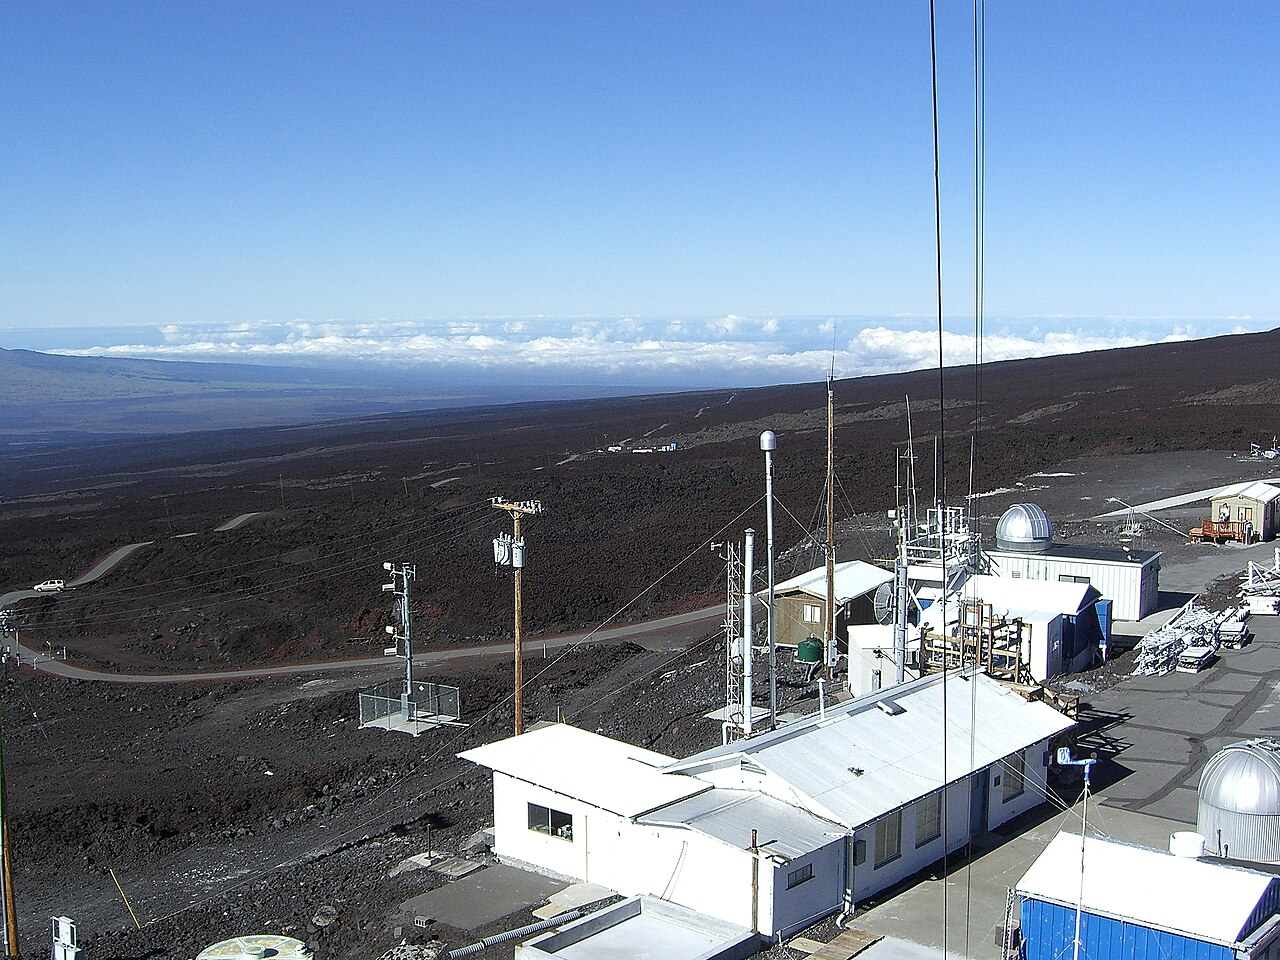
\includegraphics[width=0.56\linewidth]{images/book4/mauna-loa.jpg}\hspace{0.03\linewidth}
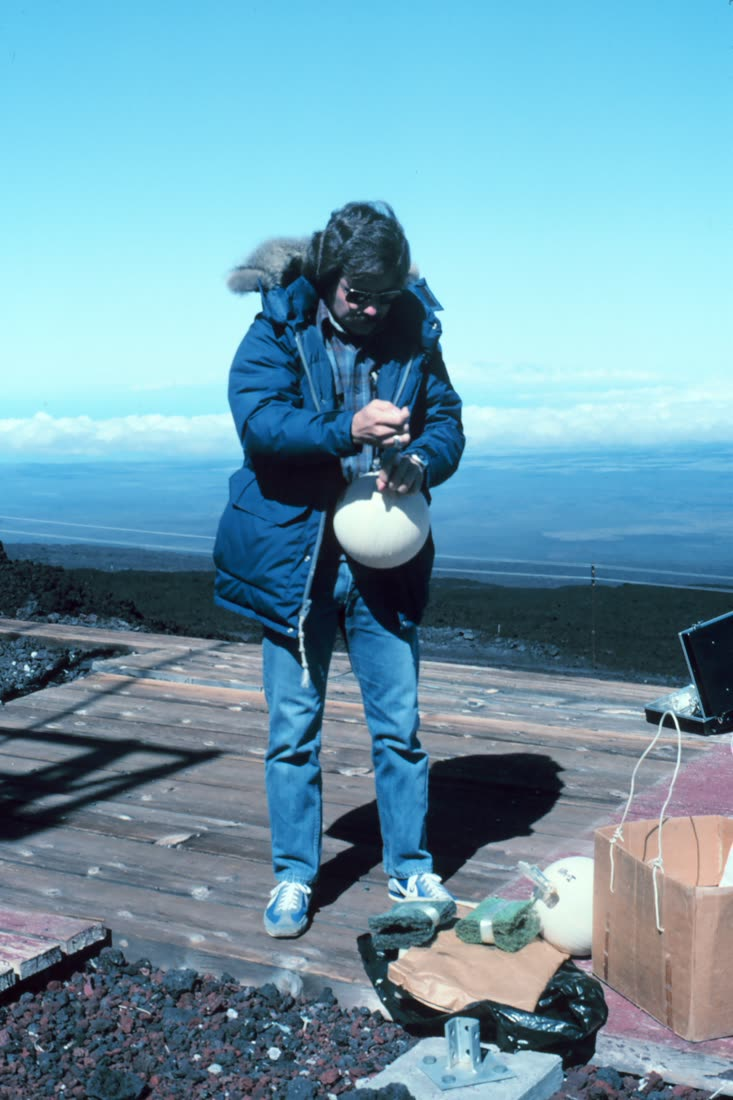
\includegraphics[width=0.33\linewidth]{images/book4/keeling-flask.jpg}

{\small Waar de curve wordt getekend. Links: het observatorium op de
noordflank van de Mauna Loa, \qty{3400}{m} hoog, boven de passaatinversie die de
eigen lucht van het eiland beneden houdt. Rechts: een luchtmonster dat in 1982
in een fles wordt genomen; zulke flessen, die in Californië worden
geanalyseerd, controleren het continue analysetoestel en worden gevuld op
stations van Alaska tot de Zuidpool.}
\end{omfigure}

\section{De stikstofkringloop}

\begin{proposition}[De stikstofkringloop]\label{prop:b2:biogeochemical-cycles:nitrogen}
\index{stikstofkringloop}\index{stikstofbinding}\index{nitrificatie}\index{denitrificatie}\index{haber-boschproces}\index{anammox}
Stikstof is overvloedig --- de lucht bevat $4\times 10^{9}$~Tg
$\mathrm{N_2}$ --- en schaars, omdat de drievoudige binding van $\mathrm{N_2}$ door
slechts twee processen wordt geopend: bliksem (enkele Tg per jaar) en
\emph{biologische \omterm{prop:b2:biogeochemical-cycles:nitrogen}{stikstofbinding}} door prokaryoten met
nitrogenase, zo'n 100 Tg per jaar op land en 100 in zee, tegen een
prijs van 16 ATP per $\mathrm{N_2}$. De gebonden stikstof doorloopt daarna een
redoxladder die door microben wordt aangedreven (\cref{ch:b2:microbial-metabolism}):
\emph{ammonificatie} van dood materiaal tot $\mathrm{NH_4^{+}}$;
\emph{nitrificatie} van $\mathrm{NH_4^{+}}$ tot $\mathrm{NO_2^{-}}$ en $\mathrm{NO_3^{-}}$ door
aerobe chemolithotrofen; opname van $\mathrm{NH_4^{+}}$ of $\mathrm{NO_3^{-}}$ door planten
en de reductie ervan terug tot amine; en, waar zuurstof ontbreekt,
\emph{\omterm{def:b2:microbial-metabolism:anaerobic}{denitrificatie}} van $\mathrm{NO_3^{-}}$ tot $\mathrm{N_2}$ (met $\mathrm{N_2O}$ als
lek) en \emph{anammox}, de anaerobe oxidatie van ammonium door
nitriet tot $\mathrm{N_2}$, die samen ongeveer evenveel aan de lucht teruggeven
als de binding opneemt. De \omterm{def:b2:biogeochemical-cycles:reservoir}{verblijftijd} van een stikstofatoom in de
biosfeer is enkele honderden jaren; in de atmosfeer $4\times
10^{9}/400 \approx 10^{7}$ jaar. Sinds 1913 bindt het \emph{haber-boschproces}
industrieel stikstof, nu ongeveer 120 Tg per jaar,
en gecultiveerde vlinderbloemigen en de verbranding van fossiele brandstoffen
voegen er 60 en 30 aan toe: menselijke activiteit bindt evenveel stikstof als
alle natuurlijke processen samen, en voedt de helft van de levende mensen.
\end{proposition}

\begin{omfigure}
\begin{tikzpicture}[every node/.style={font=\scriptsize}, >=stealth, box/.style={draw, rounded corners, minimum width=1.9cm, minimum height=0.8cm, align=center, fill=#1}]
  \node[box=omDef!15] (n2) at (0,3.4) {$\mathrm{N_2}$ in de lucht\\$4\times 10^{9}$ Tg};
  \node[box=omThm!15] (org) at (-4.6,1.0) {organisch N\\planten, bodems, zee};
  \node[box=omProp!15] (nh4) at (-2.2,-0.8) {$\mathrm{NH_4^{+}}$};
  \node[box=omProp!15] (no2) at (2.2,-0.8) {$\mathrm{NO_2^{-}}$};
  \node[box=omProp!15] (no3) at (4.6,1.0) {$\mathrm{NO_3^{-}}$};
  \draw[->, thick] (n2) -- node[above left, align=right] {binding\\nitrogenase, 200\\Haber--Bosch 120} (org);
  \draw[->, thick] (org.south) -- node[below left] {ammonificatie} (nh4.north);
  \draw[->, thick] (nh4) -- node[below] {nitrificatie} (no2);
  \draw[->, thick] (no2) -- node[below right] {nitrificatie} (no3);
  \draw[->, thick] (no3) to[bend left=18] node[above, pos=0.72] {assimilatie} (org);
  \draw[->, thick, omExo!80!black] (no3) -- node[above right, align=left] {denitrificatie\\(anoxisch), lek van $\mathrm{N_2O}$} (n2);
  \draw[->, thick, omExo!80!black] (no2) -- node[right, pos=0.55, align=left] {anammox\\(met $\mathrm{NH_4^{+}}$)} (n2);
  \node[anchor=north, align=center] at (0,-1.5) {fluxen in Tg N per jaar; elke stap behalve assimilatie en ammonificatie wordt door prokaryoten uitgevoerd};
\end{tikzpicture}

{\small De \omterm{prop:b2:biogeochemical-cycles:nitrogen}{stikstofkringloop} als redoxladder (planten assimileren
zowel ammonium als nitraat). Binding en \omterm{def:b2:microbial-metabolism:anaerobic}{denitrificatie}, de twee
deuren naar de atmosfeer, zijn allebei microbieel; de industriële deur
is nu even groot als de natuurlijke.}
\end{omfigure}

\begin{proof}[Bewijsmateriaal]
Het proefbos van Hubbard Brook, New Hampshire: in 1965 werd één volledig
stroomgebied kaalgekapt en met herbicide kaal gehouden, terwijl een naburig
stroomgebied intact bleef, en de beken die elk ervan afwateren, werden jarenlang
bemeten en geanalyseerd. Het kaalgemaakte stroomgebied verloor nitraat met
zestig keer het tempo van de controle --- het hele stikstofkapitaal van de
bodem, dat niet meer door planten werd opgenomen, werd genitrificeerd en
uitgespoeld, nam calcium en kalium mee en verzuurde de beek. Het experiment
toonde hoe gesloten de kringloop in een intact bos is (enkele kilogrammen
stikstof verloren per hectare per jaar, tegenover honderden die rondgaan) en
wat hem doorbreekt.
\end{proof}

\section{Fosfor en zwavel}

\begin{proposition}[Twee kringlopen zonder snel gas]\label{prop:b2:biogeochemical-cycles:ps}
\index{fosforkringloop}\index{zwavelkringloop}\index{eutrofiëring}\index{dimethylsulfide}
\emph{Fosfor} heeft geen gasvorm. Het komt ecosystemen binnen door de
verwering van apatiet in gesteente, zo'n 20 Tg per jaar over het hele
landoppervlak, wordt binnen bodems en meren vele malen gerecycled
--- een fosfaation in het oppervlaktewater van een meer wordt binnen enkele
uren opgenomen --- en vertrekt naar de sedimenten, waar het de
$10^{8}$ jaar van een gesteentekringloop blijft. Het leven is daarom zuinig met
fosfor en fosforgelimiteerd: de \omterm{def:b2:biogeochemical-cycles:reservoir}{verblijftijd} in de oceaan is zo'n
\num{20000} jaar, en het fosfaat van de diepzee, dat door opwelling naar
boven komt, bepaalt de productiviteit ervan. Mijnbouw brengt nu ongeveer
evenveel fosfor op landbouwgrond als verwering vrijmaakt, en de afspoeling
ervan naar meren veroorzaakt \emph{eutrofiëring}: een algenbloei, de afbraak
ervan, het verbruik van zuurstof, en de dood van de vissen --- de experimenten
van Schindler met hele meren in Ontario in de jaren 1970, waarbij de ene helft
van een meer met fosfor werd bemest en de andere niet, toonden aan dat fosfor
alleen de trigger is, en leidden tot de verwijdering ervan uit wasmiddelen.
\emph{Zwavel} heeft zowel een gesteentekringloop (gips, pyriet) als een
gasfase: het $\mathrm{SO_2}$ van vulkanen en steenkool, het $\mathrm{H_2S}$ van
anoxische sedimenten, en \emph{\omterm{prop:b2:biogeochemical-cycles:ps}{dimethylsulfide}} uit marien plankton, waarvan de
oxidatieproducten de wolken boven de oceaan kiemen leveren. Het verbranden van
steenkool verdrievoudigde in de twintigste eeuw de zwavelflux naar de lucht en
bezorgde Europa en Noord-Amerika hun zure regen; rookgasreinigers keerden dat
binnen enkele decennia om, omdat de \omterm{def:b2:biogeochemical-cycles:reservoir}{verblijftijd} van de kringloop in de lucht
maar enkele dagen is.
\end{proposition}

\begin{omfigure}
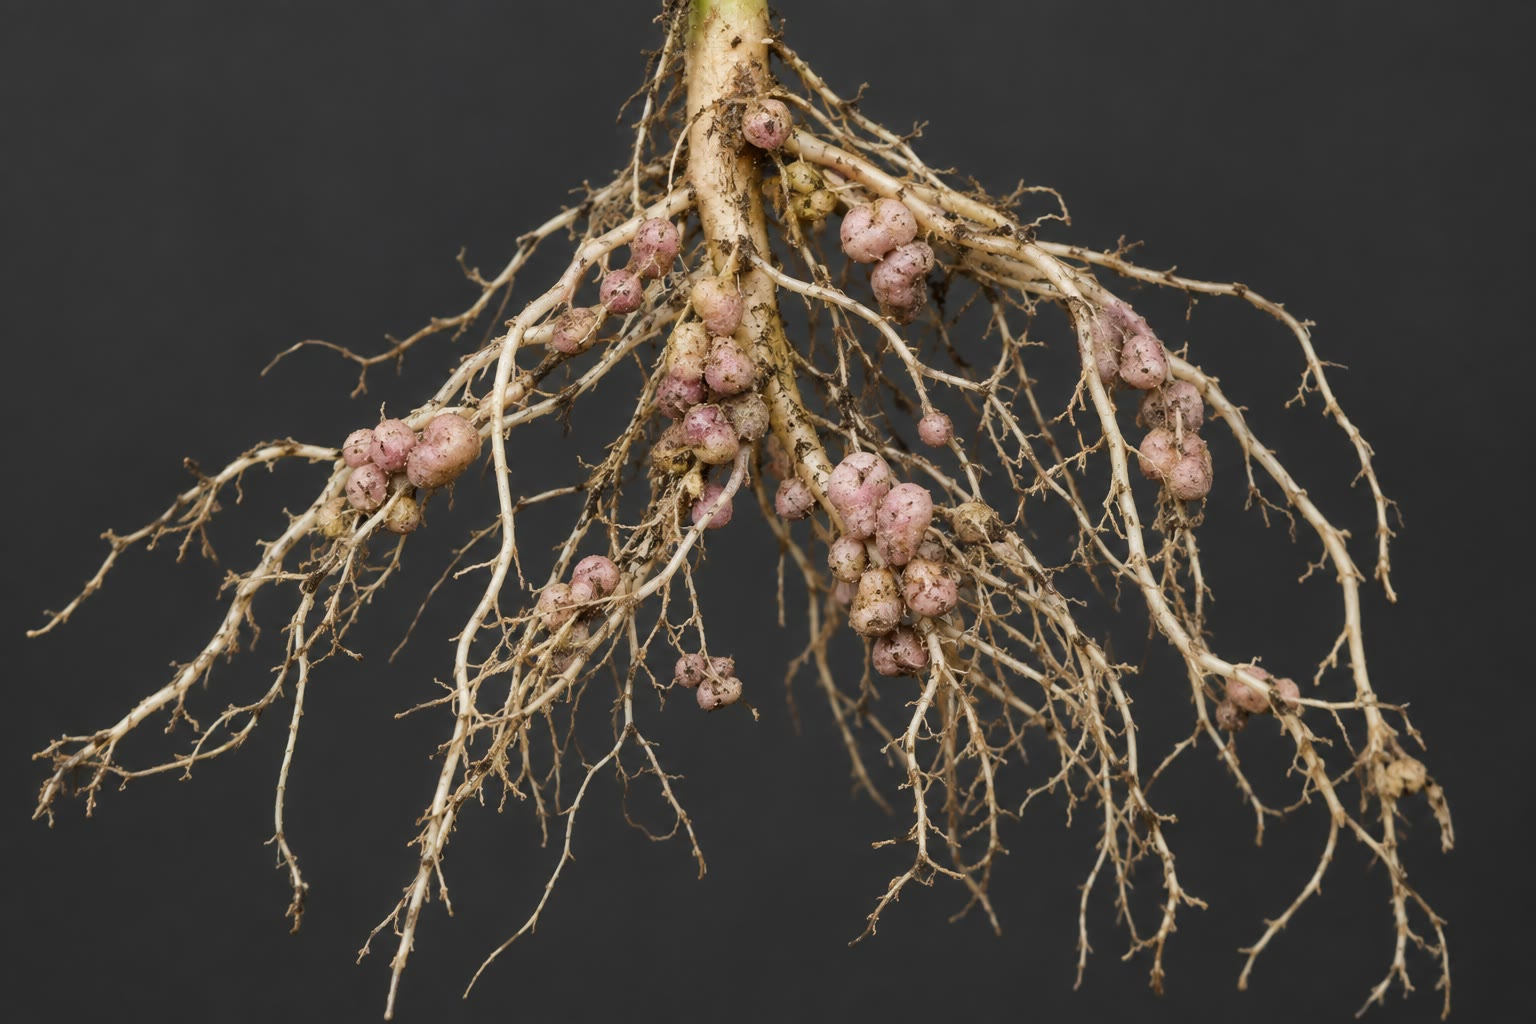
\includegraphics[width=0.44\linewidth]{images/book4/ai/b4-25-root-nodules.jpg}\hspace{0.04\linewidth}
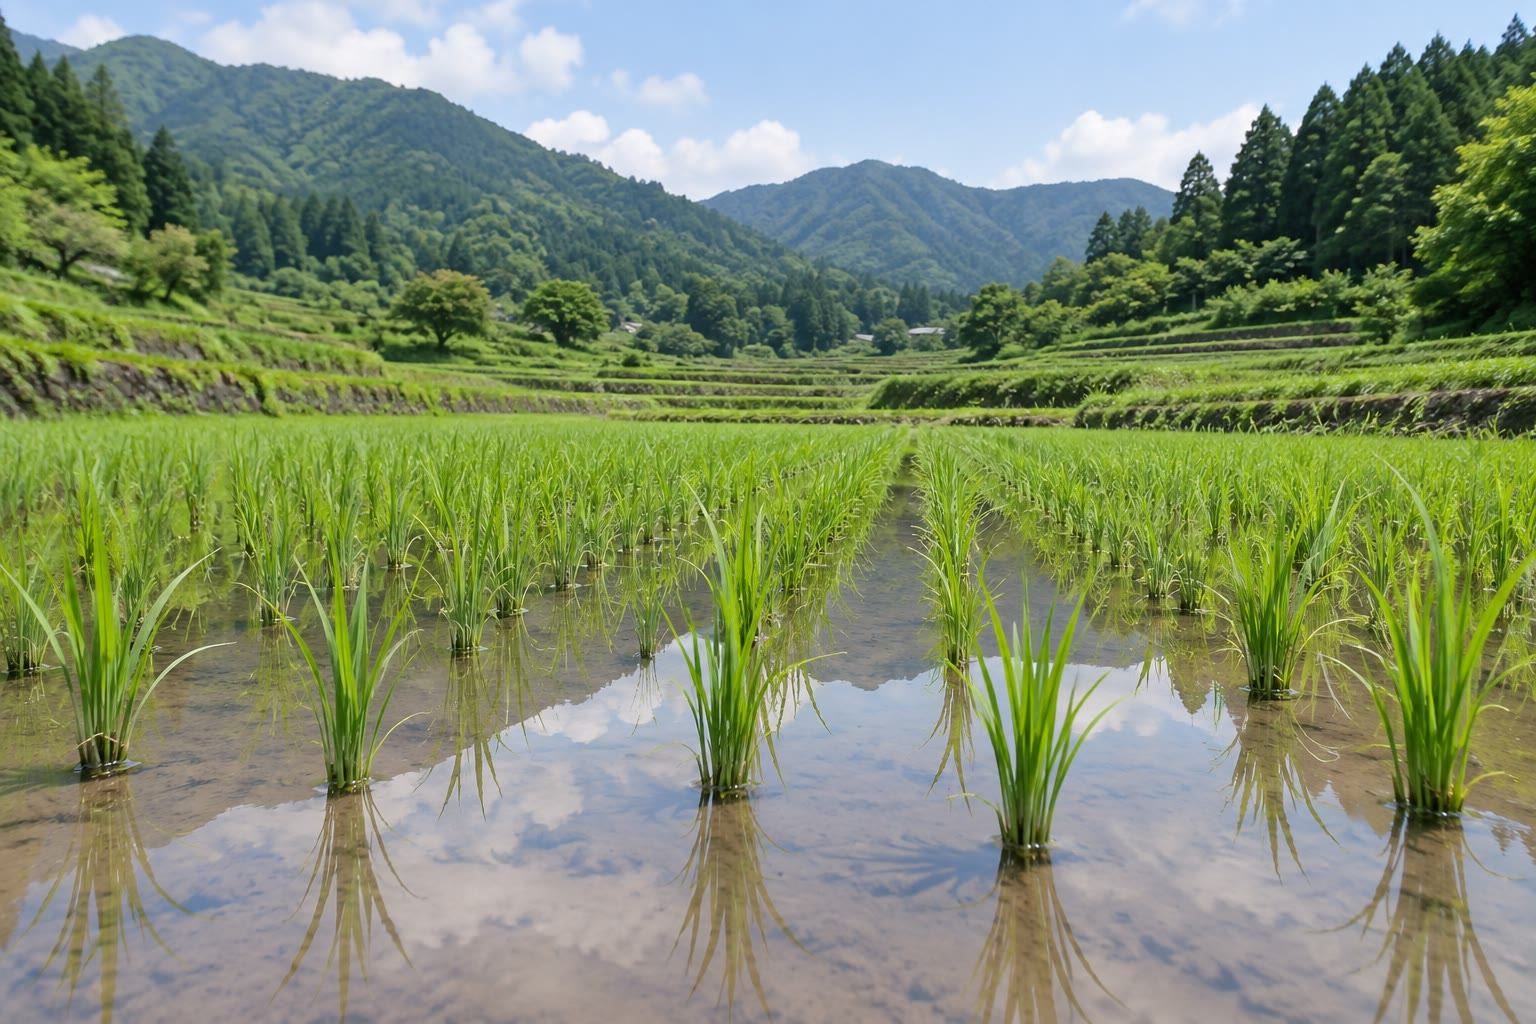
\includegraphics[width=0.44\linewidth]{images/book4/ai/b4-25-rice-paddy.jpg}

{\small Twee deuren van de \omterm{prop:b2:biogeochemical-cycles:nitrogen}{stikstofkringloop}. Links: wortelknolletjes van een
vlinderbloemige, elk een kamertje waarin rhizobia stikstof binden voor hun
gastheer. Rechts: een ondergelopen rijstveld, anoxisch onder het oppervlak,
waar \omterm{def:b2:microbial-metabolism:anaerobic}{denitrificatie} stikstof aan de lucht teruggeeft en methanogenen methaan
maken.}
\end{omfigure}

\section{De verstoorde planeet}

\begin{example}[Wat de getallen zeggen]\label{ex:b2:biogeochemical-cycles:numbers}
Een uitstoot van \qty{10}{GtC} per jaar met een \omterm{prop:b2:biogeochemical-cycles:carbon}{atmosferische fractie} van
$0.45$ laat elk jaar \qty{4.5}{GtC}, of \qty{2.1}{ppm}, in de lucht achter
--- de waargenomen helling. De cumulatieve uitstoot sinds 1850 is ongeveer
\qty{700}{GtC}, waarvan \qty{290}{GtC} in de lucht zit (140~ppm), de
rest in oceaan en land. Om de atmosfeer op welk niveau ook te houden, moet de
netto-uitstoot dalen tot wat de trage putten --- menging naar de diepe oceaan
en verwering, samen minder dan \qty{1}{GtC} per jaar --- kunnen opnemen:
\emph{netto nul} is geen slogan maar de voorwaarde voor \omterm{def:b2:biogeochemical-cycles:reservoir}{stationaire toestand} van
het \omterm{thm:b2:biogeochemical-cycles:box}{boxmodel} met een zeer lange $\tau$. Voor stikstof heeft de verdubbeling van
de \omterm{def:b2:biogeochemical-cycles:reservoir}{flux} van gebonden stikstof het nitraat in rivieren verdubbeld, dode zones
veroorzaakt bij de monding van de Mississippi en in de Oostzee, en het
$\mathrm{N_2O}$ van de atmosfeer, een broeikasgas met een \omterm{def:b2:biogeochemical-cycles:reservoir}{verblijftijd}
van een eeuw, met een vijfde verhoogd. \Cref{ch:b2:global-change} volgt
de gevolgen voor levende wezens.
\end{example}

\section{Opgaven}

\begin{exercise}[$\star$]\label{exo:b2:biogeochemical-cycles:1}
Definieer \omterm{def:b2:biogeochemical-cycles:reservoir}{reservoir}, \omterm{def:b2:biogeochemical-cycles:reservoir}{flux} en \omterm{def:b2:biogeochemical-cycles:reservoir}{verblijftijd}, en bereken de \omterm{def:b2:biogeochemical-cycles:reservoir}{verblijftijd} van
koolstof in landplanten (450 GtC, fotosynthese 120 GtC per jaar) en in de
diepe oceaan (\num{37000} GtC, uitwisseling ongeveer 100 GtC per jaar).
\end{exercise}

\begin{exercise}[$\star$]\label{exo:b2:biogeochemical-cycles:2}
Reken \qty{2.5}{ppm} per jaar om in GtC, en \qty{10}{GtC}
uitstoot in ppm.
\end{exercise}

\begin{exercise}[$\star$]\label{exo:b2:biogeochemical-cycles:3}
Noem de twee natuurlijke processen die $\mathrm{N_2}$ openen, het proces dat
het teruggeeft, en de drie redoxstappen daartussen, met de
verantwoordelijke organismen.
\end{exercise}

\begin{exercise}[$\star$]\label{exo:b2:biogeochemical-cycles:4}
Waarom beperkt fosfor over geologische tijd vaker de productiviteit dan
stikstof, en stikstof vaker dan fosfor binnen een
seizoen?
\end{exercise}

\begin{exercise}[$\star\star$]\label{exo:b2:biogeochemical-cycles:5}
Een meer van \qty{e7}{m^3} ontvangt \qty{2}{t} fosfor per jaar
en ververst jaarlijks \qty{20}{\%} van zijn water. Bereken de
fosforconcentratie in \omterm{def:b2:biogeochemical-cycles:reservoir}{stationaire toestand} en de tijd om \qty{90}{\%}
daarvan te bereiken nadat de aanvoer begint. En als de aanvoer wordt gehalveerd?
\end{exercise}

\begin{exercise}[$\star\star$]\label{exo:b2:biogeochemical-cycles:6}
Bereken uit de gegevens van Keeling de gemiddelde groeisnelheid van $\mathrm{CO_2}$ in
de jaren 1960 (316 tot \qty{325}{ppm} over tien jaar) en in de jaren 2010
(390 tot 411 over negen jaar), in ppm per jaar en in GtC per jaar.
\end{exercise}

\begin{exercise}[$\star\star$]\label{exo:b2:biogeochemical-cycles:7}
De seizoenszaagtand op de Mauna Loa heeft een amplitude van ongeveer
\qty{6}{ppm} van piek tot dal. Reken om in GtC en vergelijk met de
jaarlijkse netto primaire productie van het land op het noordelijk halfrond,
ongeveer \qty{35}{GtC}. Waarom is de zaagtand zoveel kleiner?
\end{exercise}

\begin{exercise}[$\star\star$]\label{exo:b2:biogeochemical-cycles:8}
Nitrogenase besteedt 16 ATP per $\mathrm{N_2}$. Bereken voor een vlinderbloemige
die \qty{200}{kg} stikstof per hectare per jaar bindt de mol
$\mathrm{N_2}$ gebonden en het bestede ATP, en de massa glucose die dat ATP
vertegenwoordigt (ongeveer 30 ATP per glucose). Welke fractie van de
fotosyntheseproducten van een gewas van \qty{10}{t/ha} is dat?
\end{exercise}

\begin{exercise}[$\star\star$]\label{exo:b2:biogeochemical-cycles:9}
Plankton groeit volgens de redfieldverhouding $\mathrm{C:N:P} = 106:16:1$.
Zeewater in de diepte bevat \qty{2.2}{\micro mol/kg} fosfaat en
\qty{32}{\micro mol/kg} nitraat. Welk van beide raakt eerst op wanneer een
waterpakket naar het oppervlak wordt gebracht, en hoeveel koolstof wordt er
gebonden voordat dat gebeurt?
\end{exercise}

\begin{exercise}[$\star\star\star$]\label{exo:b2:biogeochemical-cycles:10}
Behandel de atmosfeer als een box met een koolstofoverschot $E$ dat met snelheid
$E/\tau$ door de putten wordt verwijderd en door een uitstoot $Q$ wordt gevoed.
Wat is met $\tau =
50$ jaar en $Q = \qty{10}{GtC/yr}$ het overschot in \omterm{def:b2:biogeochemical-cycles:reservoir}{stationaire toestand}, en met
hoeveel ppm komt dat overeen? Leg uit waarom het echte antwoord slechter is.
\end{exercise}

\begin{exercise}[$\star\star\star$]\label{exo:b2:biogeochemical-cycles:11}
Kernproeven verdubbelden in 1963 het $\mathrm{{}^{14}C}$ van de atmosfeer; het
overschot halveerde daarna ongeveer elke 11 jaar, hoewel $\mathrm{{}^{14}C}$
een halveringstijd van 5730 jaar heeft. Leg uit wat er werd gemeten, en wat
die 11 jaar over de koolstofkringloop zegt.
\end{exercise}

\begin{exercise}[$\star\star\star$]\label{exo:b2:biogeochemical-cycles:12}
``De mens heeft de \omterm{prop:b2:biogeochemical-cycles:nitrogen}{stikstofkringloop} verdubbeld en de koolstofkringloop slechts
een duwtje gegeven.'' Bespreek dit met getallen: gebonden \omterm{def:b2:biogeochemical-cycles:reservoir}{fluxen}, fracties van
de natuurlijke \omterm{def:b2:biogeochemical-cycles:reservoir}{flux}, en de getroffen \omterm{def:b2:biogeochemical-cycles:reservoir}{reservoirs}.
\end{exercise}

\section{Vraagstuk: het koolstofbudget van een eeuw}

\begin{problem}[{Weekendvraagstuk --- een eeuw uitstoot door het boxmodel van
de atmosfeer gehaald, het aandeel van de oceaan en dat van het land, de
stikstofcascade van een bemest veld tot een dode zone, en het fosforbudget van
een meer, met als besluit de atmosferische fractie, de atmosferische
concentratie in 2100 en de stikstof die per hectare verloren gaat}]
\label{pb:b2:biogeochemical-cycles:1}
Gegevens. Atmosfeer in 1850: \qty{285}{ppm}; \qty{1}{ppm} $=
\qty{2.13}{GtC}$. Cumulatieve uitstoot 1850--2020: \qty{700}{GtC};
atmosferisch $\mathrm{CO_2}$ in 2020: \qty{412}{ppm}. Een veld van
\qty{1}{ha} krijgt \qty{150}{kg} stikstofmest per jaar;
het gewas neemt \qty{60}{\%} op, \qty{25}{\%} wordt gedenitrificeerd, de
rest spoelt uit. Een meer van \qty{5e7}{m^3} ververst een tiende van zijn water
per jaar en ontvangt \qty{5}{t} fosfor per jaar.

\medskip
\noindent\textbf{Deel I --- De \omterm{prop:b2:biogeochemical-cycles:carbon}{atmosferische fractie}.}
\begin{enumerate}
  \item Bereken de atmosferische koolstof in 1850 en in 2020, en de
        toename in GtC.
  \item Bereken de \omterm{prop:b2:biogeochemical-cycles:carbon}{atmosferische fractie} over 1850--2020.
  \item Waar is de rest? Geef de twee putten en, uit de
        propositie, hun geschatte aandelen.
  \item Als de oceaan \qty{25}{\%} van de uitstoot heeft opgenomen, met hoeveel
        is haar opgeloste anorganische koolstof, \qty{38000}{GtC}, dan relatief
        gestegen? Waarom verzuurt de oppervlakte-oceaan toch meetbaar?
  \item Waarom blijft de \omterm{prop:b2:biogeochemical-cycles:carbon}{atmosferische fractie} ruwweg constant terwijl de
        uitstoot exponentieel groeit? (Beschouw het \omterm{thm:b2:biogeochemical-cycles:box}{boxmodel} met
        $Q \propto e^{t/T}$ en een put $E/\tau$.)
  \item Wat zou de \omterm{prop:b2:biogeochemical-cycles:carbon}{atmosferische fractie} worden als de uitstoot eeuwenlang
        constant werd gehouden?
\end{enumerate}

\medskip
\noindent\textbf{Deel II --- De komende eeuw.}
Modelleer het koolstofoverschot $E$ (boven het niveau van 1850) met
$\mathrm{d}E/\mathrm{d}t = Q - E/\tau$, $\tau = 100$ jaar.
\begin{enumerate}[resume]
  \item Bereken het overschot in 2020 in GtC.
  \item Bereken met $Q$ constant op \qty{10}{GtC/yr} het overschot in
        \omterm{def:b2:biogeochemical-cycles:reservoir}{stationaire toestand} en de concentratie die daaruit volgt.
  \item Los $E(t)$ op vanaf 2020 met $Q = 10$ en geef $E$ in
        2100 en de concentratie.
  \item Laat $Q$ nu tussen 2020 en 2070 lineair dalen tot nul en daarna
        nul blijven. Bereken $E$ in 2070 (integreer de vergelijking;
        de particuliere oplossing voor een lineaire $Q$ is lineair plus een
        constante) en in 2100.
  \item Vergelijk de twee concentraties in 2100.
  \item Waarom is één enkele $\tau$ optimistisch voor het tweede scenario?
\end{enumerate}

\medskip
\noindent\textbf{Deel III --- De stikstofcascade.}
\begin{enumerate}[resume]
  \item Bereken de stikstof die per hectare per jaar door het gewas wordt
        opgenomen, wordt gedenitrificeerd en uitspoelt.
  \item De uitgespoelde stikstof bereikt als nitraat een rivier en daarna de
        zee, waar plankton haar volgens de redfieldverhouding gebruikt. Hoeveel
        koolstof laat ze het plankton binden?
  \item Die koolstof zakt uit en wordt in de diepte geademd, waarbij
        zuurstof wordt verbruikt met 1 $\mathrm{O_2}$ per C. Bereken de verbruikte
        zuurstof in mol en in kilogram.
  \item Een kubieke meter zeewater bevat verzadigd ongeveer \qty{0.25}{mol}
        $\mathrm{O_2}$. Hoeveel kubieke meter bodemwater
        ontdoet de uitspoeling van één hectare van zuurstof?
  \item De gedenitrificeerde fractie ontsnapt deels als $\mathrm{N_2O}$,
        \qty{1}{\%} van de gedenitrificeerde stikstof. Bereken het $\mathrm{N_2O}$
        per hectare per jaar, en zijn opwarmingsequivalent in $\mathrm{CO_2}$
        ($\mathrm{N_2O}$ is per kilogram 270 keer $\mathrm{CO_2}$).
  \item Vergelijk met het $\mathrm{CO_2}$ dat werd uitgestoten om de mest te maken
        (ongeveer \qty{4}{kg} $\mathrm{CO_2}$ per kilogram stikstof via
        Haber--Bosch).
\end{enumerate}

\medskip
\noindent\textbf{Deel IV --- Het meer.}
\begin{enumerate}[resume]
  \item Bereken de \omterm{def:b2:biogeochemical-cycles:reservoir}{verblijftijd} van fosfor in het meer als verversing het
        enige verlies is, en de concentratie in \omterm{def:b2:biogeochemical-cycles:reservoir}{stationaire toestand} in
        \unit{mg/m^3}.
  \item Meren met meer dan \qty{30}{mg/m^3} fosfor zijn
        eutroof. Is dit meer dat?
  \item Sedimentatie verwijdert fosfor met een eigen tijdconstante
        van 5 jaar. Bereken de \omterm{def:b2:biogeochemical-cycles:reservoir}{verblijftijd} en de concentratie opnieuw.
  \item De aanvoer wordt teruggebracht tot \qty{1}{t} per jaar. Bereken de nieuwe
        \omterm{def:b2:biogeochemical-cycles:reservoir}{stationaire toestand} en de tijd om er tot op \qty{10}{\%} bij te komen.
  \item Waarom herstellen veel meren trager dan deze berekening
        voorspelt?
  \item Bereken de koolstof die de fosfor van het meer elk jaar volgens de
        redfieldverhouding in plankton kan inbouwen, uit de aanvoer van
        \qty{5}{t}.
  \item Formuleer het resultaat: de \omterm{prop:b2:biogeochemical-cycles:carbon}{atmosferische fractie}, de twee
        concentraties in 2100, en de stikstof die per hectare
        uitspoelt.
\end{enumerate}
\end{problem}
